\documentclass[12pt,a4paper,headinclude,twoside, plainheadsepline, open=right,numbers=noenddot]{scrreprt}

%%
%
%%%%%%%%%%%%%%%%%%%%%%%%%%%%%%%%%%%%%%%%%%%%%%%%%%%%%%%%%%%
%
% Literaturverzeichnis
%
% Hier eine von zwei Varianten auswaehlen:
% Nummern oder Buchstaben fuer Referenzen
%\usepackage[backend=biber, style=alphabetic, sorting=nyt]{biblatex}
\usepackage[backend=biber, style=numeric-comp, sorting=none]{biblatex}
\usepackage{multicol}
%\usepackage[onehalfspacing]{setspace}
\usepackage{mathtools}
\usepackage{pxfonts}
\usepackage{pdfpages}
%
% Hier werden die Referenzen in einer separaten Datei gespeichert
\addbibresource{Laborpraktikum.bib}
%
% WICHTIG: Hier wird nicht BibTeX sondern BibLateX verwendet!!
% Deshalb nicht mit bibtex uebersetzen, sondern mit biber
% Das kann man in jedem Tool wie TexMaker oder TexShop als Option einstellen
%

% Spezielle Einstellungen, insbesondere fuer das Literaturverzeichnis,
% aber auch Packages wie amsmath, Groessenanpassungen etc.
\input{./Preferences.tex}

\begin{document}
\pagenumbering{Roman} % grosse Roemische Seitenummerierung
\pagestyle{empty}

%%%%%%%%%%%%%%%%%%%%%%%%%%%%%%%%%%%%%%%%%%%%%%%%%%%%%%%%%%%%%%%%%%%%%
% Titelseite
\clearscrheadings\clearscrplain

\begin{titlepage}
\begin{figure}[thb]
       \includegraphics[height=2.5cm]{./Images/FakIM_Vorlage_Logo_Vektor.eps}
\end{figure}
\begin{center}
\rule{0pt}{0pt}
\vfill

\begin{huge}
Emotion Recognition\\[0.75ex]
\end{huge}
\begin{large}
P2 - Deep Learning Eye Catcher
\end{large}


\vfill
\vfill

Bericht zum Laborpraktikum\\
im Sommersemester 2019 von\\
\vfill
\setlength{\columnsep}{.0cm}
\begin{multicols}{1}

\textbf{Lukas Schulz}\\
Matrikelnummer: 3042081

\textbf{Noor Alrabea}\\
Matrikelnummer: 3103436
\end{multicols}

\begin{multicols}{2}
\textbf{Markus Hofer}\\
Matrikelnummer: 123456789

\textbf{Benjamin Bauer}\\
Matrikelnummer: 3092255
\end{multicols}

\begin{multicols}{2}
\textbf{Mona Ziegler}\\
Matrikelnummer: 3091609

\textbf{Anna Will}\\
Matrikelnummer: 3086698
\end{multicols}

\begin{multicols}{2}
\textbf{Julia Karnaukh}\\
Matrikelnummer: 12345678

\textbf{David Wolf}\\
Matrikelnummer: 12345678
\end{multicols}

\vfill
\vfill
\textbf{\large Fakult"at Informatik und Mathematik\\
Ostbayerische Technische Hochschule Regensburg\\
(OTH Regensburg)}
\vfill
\vfill

\begin{tabular}{rl}
Pr"ufer:   & Prof. Dr. Christoph Palm\\
Abgabedatum:& 25. Juni 2019
\end{tabular}
\end{center}
\end{titlepage}


\pagestyle{useheadings} % normale Kopf- und Fusszeilen fuer den Rest
\tableofcontents % Inhaltsverzeichnis


\chapter{Einleitung}
\label{einleitung}
\pagenumbering{arabic} % ab jetzt arabische Nummerierung

\section{Motivation und Einführung}
Künstliche Intelligenz ist bereits in vielen Situationen des Lebens alltäglich geworden. So steckt hinter der Gesichtserkennung im Smartphone oder Sprachassistenten wie Amazons "{}Alexa"{} Künstliche Intelligenz. Der große Vorteil und Nutzen an KI liegt vor allem in der Mustererkennung und Zuordnung zu vorgegebenen Kategorien. In der Medizin spielt das vor allem bei der Verarbeitung der Ergebnisse Bildgebender Diagnoseverfahren eine große Rolle. Eine KI kann Muster in beispielsweise Röntgenbildern erkennen, und so den Arzt bei der Diagnosefindung unterstützen.
Daran wird auch im Labor des ReMIC (Regensburg Medical Image Computing) geforscht und verschiedene Anwendungen zur Bildanalyse entwickelt. Hierbei liegt der Fokus immer mehr auf Deep-Learning Ansätzen. Um nun mehr interessierte Studierende der OTH über diese Tätigkeit zu informieren, soll eine einfache Deep-Learning Anwendung zur Emotionserkennung entwickelt werden. Um so viele Studierende wie möglich dafür zu begeistern, wurde entschieden, ein Spiel zu entwickeln. 

\section{Das Programm}
Neben der Tür des ReMIC gibt es ein "{}Schaufenster"{}, hinter diesem ist ein Bildschirm aufgebaut, der im Moment genutzt wird um allgemeine Informationen über das Labor anzuzeigen. In Zukunft soll dort zwischen den Vorlesungszeiten das entwickelte Programm spielbar sein. Hierfür wird eine Kamera über den Bildschirm aufgebaut. 
\\
Das Spiel wird gestartet, wenn das Gesicht eines Spielers in einem ausgewiesenen Bereich erkannt wurde. Dem Spieler wird nun eine zufällig ausgewählte Emotion vorgegeben, die er nun nachmachen soll. Das Programm ist in der Lage sieben Emotionen zu erkennen:  Neutral, Angewidert, Wütend, Glücklich, Überrascht, Traurig, Ängstlich. Die erreichte Punktzahl pro Runde ergibt sich daraus, wie gut die Emotion durch das Programm erkannt werden konnte. Die höchste pro Runde erreichbare Punktzahl ist 100, für eine zu 100\% erkannte Emotion. \\ Falls kein oder mehrere Gesichter erkannt wurden, soll eine Fehlermeldung auf dem Bildschirm ausgegeben werden. \\ Das Spiel endet, wenn der Spieler den von der Kamera erfassten Bereich verlässt. Danach werden die Bilddaten des Spielers gelöscht. 
%Fehlermeldungen wenn kein oder mehrere Gesichter erkannt werden


\section{Künstliche Intelligenz und Deep Learning}
% Eine Künstliche Intelligenz soll in der Lage sein, Problemstellungen, die der Mensch intuitiv lösen würde, auf eine ähnliche Art und Weise lösen zu können. 
Traditionell liegen die Stärken einer Maschine bei rechenaufwändigen, für den Menschen kaum oder nur sehr langsam lösbare Aufgaben. Auch große Datenmengen stellen dabei für einen Computer keine große Herausforderung dar. Im Gegensatz dazu sind Probleme, die der Mensch intuitiv oder situationsabhängig lösen würde, durch konventionelle Programmierung kaum erfassbar. Der Programmierer müsste jede mögliche Situation abfangen, in vielen Fällen ist dies aufgrund des Umfangs nicht effizient umsetzbar. Bei der Emotionserkennung  beispielsweise hat der Mensch keine Schwierigkeiten, in verschiedenen Gesichtern Emotionen zu erkennen und zu unterscheiden, obwohl sich die Ausprägung verschiedener Merkmale dabei in jedem Gesicht stark unterscheiden kann. Um eine solche Aufgabe maschinell lösen zu können, wird die Verwendung einer künstlichen Intelligenz notwendig. 
\paragraph{}
Ein Vielversprechender Ansatz zur Entwicklung einer künstlichen Intelligenz ist das Deep Learning. Dabei werden neue, komplexe Probleme gelöst indem sie aus bekannten, einfachen Problemen zusammengesetzt werden. Hierfür werden neuronale Netze verwendet. Diese sind vom Aufbau und der Struktur der Verschaltung des menschlichen Gehirn nachempfunden. Es gibt Knotenpunkte (= Neuronen), die mit anderen Knotenpunkten verbunden sind, und so Informationen weitergeben. Beim Deep Learning sind diese Knoten in Schichten angeordnet. Die erste Schicht ist sichtbar, und umfasst die rohen Eingangsdaten. Diese werden abstrahiert, auf eine nächste versteckte Schicht abgebildet, wieder verarbeitet und an die nächste Schicht weitergegeben. Dies geschieht einige Male, bis die Daten an die letzte Ebene weitergegeben werden. Dort erhält man ein prozentuales Ergebnis, zu welcher Kategorie die Eingangsdaten zugeordnet werden können. Wie genau die versteckten Schichten arbeiten, an welchen Punkten sie sich orientieren, oder worauf die letztendliche Entscheidung basiert, ist von außen nicht ersichtlich. Die internen Parameter müssen nicht von einem Programmierer festgelegt werden, sondern werden vom neuronalen Netz selbst über ein Trainingsverfahren gelernt \cite{Goodfellow-et-al-2016}. 
\paragraph{}
Zum Training wird in der Praxis meist Supervised Learning angewendet. Dabei werden neben den Daten, die in eine Kategorie eingeordnet werden sollen, auch der gewünschte Output übergeben. Nun sollen die internen Parameter so angepasst werden, dass sich der Fehler minimiert. Um dieses Minimum zu finden, wird häufig das Gradientenabstiegsverfahren verwendet. Hierfür berechnet der Lernalgorithmus für jeden Parameter einen Gradienten, der angibt, in wie weit sich der fehlerhafte Output verbessert oder verschlechtert, falls der Parameter leicht erhöht wird. Der Parametervektor wird dann in die entgegengesetzte Richtung zum Gradienten angepasst, um so einen minimalen Wert für den Fehler zu erhalten \cite{LeCun2015DeepLearning}. 

%Automatische Emotionserkennung als Überschrift
\chapter{Automatische Emotionserkennung}
\label{Automatische Emotionserkennung}
Mimiken entstehen durch die Kontraktion verschiedener Gesichtsmuskeln, welche zu den Änderungen der jeweiligen Gesichtsmerkmale führen. So kommt es zum Beispiel zum Zusammenkneifen der Augenlider, Heben der Augenbrauen und Lippen oder Hochziehen der Nase. Durch das Auftreten von Grübchen und Fältchen kann sich auch die Textur der Haut verändern. Verschiedene Emotionen führen zu unterschiedlichen charakteristischen Änderungen im Gesicht, wobei manche Emotionen schwieriger zu erkennen sind als andere. Wir beschäftigen uns hier mit den sechs Basis Emotionen: Freude, Trauer, Angst, Ekel, Überraschung und Wut \cite{Fasel2002AutomaticFacialExpressionsAnalysis}. Wichtig um diese Emotionen zu erkennen sind die Lage, Intensität und Dynamik der entscheidenden Merkmale \cite{Fasel2002AutomaticFacialExpressionsAnalysis}. \\
Um Emotionen automatisch erkennen zu können müssen drei grundlegende Phasen durchlaufen werden. Als erstes muss das Gesicht und dessen Komponenten erkannt werden, dann müssen die Merkmale extrahiert und letztendlich als ein Ausdruck klassifiziert werden \cite{Ko2018FacialEmotionRecognition}.

\section{Gesichtsdetektion}
Der erste Schritt für eine funktionierende Emotionserkennung ist die richtige Detektion des Gesichts. Im besten Fall enthält ein Emotionserkennungsprogramm einen Gesichtsdetektor, der es erlaubt ein Gesicht in komplexen Szenen mit einem schwierigen Hintergrund zu erkennen. Manche Methoden zur Emotionserkennung brauchen die exakte Position des Gesichts, bei anderen, wie beim Active Appearance Modell reicht die grobe Lokalisierung \cite{Fasel2002AutomaticFacialExpressionsAnalysis}.\\
Bei der Detektion des Gesichts kann man zwischen Merkmal und Bild basierten Methoden unterscheiden. Ersteres eignet sich gut für Echtzeitsysteme bei denen Farbe und Bewegung beteiligt ist, letzteres ist eine stabile Technik für statische Grauwertbilder \cite{Hjelmas2001FaceDetection}. \\
Die Entwicklung des merkmalsbasierten Ansatzes kann man weiter in drei Bereiche unterteilen: die Low-Level Analyse, Merkmalsanalyse und der Verwendung aktiver Formmodelle. Die Low-Level Analyse befasst sich zunächst mit der Segmentierung visueller Merkmale unter Verwendung von Pixeleigenschaften wie Graustufen und Farben. Allerdings sind aufgrund der niedrigen Ebene die aus dieser Analyse generierten Merkmale nicht eindeutig. Deshalb macht man als nächstes eine Merkmalsanalyse, bei der visuelle Merkmale, unter Verwendung von Informationen zur Gesichtsgeometrie, zu einem globaleren Konzept des Gesichts und der Gesichtsmerkmale organisiert. Dadurch wird die Mehrdeutigkeit von Merkmalen reduziert und die Position von Gesicht beziehungsweise Gesichtsmerkmalen bestimmt. Der letzte Schritt umfasst die Verwendung aktiver Formmodelle von Schlangen bis hin zu neueren Punktverteilten Modellen (PDM) \cite{Hjelmas2001FaceDetection}.\\
Beim bildbasierten Verfahren wird eine Fensterabtasttechnik zum Erfassen von Gesichtern angewendet \cite{Hjelmas2001FaceDetection}. Der Fensterabtastalgorithmus ist im Wesentlichen nur eine Suche auf dem Eingabebild nach in allen Maßstäben möglichen Gesichtsorten, wobei es Unterschiede bei der Implementierung dieses Algorithmus für fast alle bildbasierten Systeme gibt. Typischerweise variieren die Größe des Abtastfensters, die Unterabtastrate, die Schrittgröße und die Anzahl der Iterationen in Abhängigkeit von dem vorgeschlagenen Verfahren und der Notwendigkeit eines rechnerisch effizienten Systems \cite{Hjelmas2001FaceDetection}.

\section{Merkmal Extrahierung}
Hat man das Gesicht einmal detektiert, geht es daran die Merkmale zu extrahieren. Man kann sich hierbei auf das gesamte Gesicht oder nur bestimmte Teilbereiche beziehen \cite{Fasel2002AutomaticFacialExpressionsAnalysis}. Um Gesichtsausdrücke aus einem frontal aufgenommenen Bild zu erkennen, muss eine Reihe von Schlüsselparametern, die die Gesichtsausdrücke am besten beschreiben, aus dem Bild erarbeitet werden. Diese Parameter, auch Merkmalsvektor genannt, werden genutzt, um später zwischen den verschiedenen Emotionen unterscheiden zu können. Der wichtigste Aspekt einer erfolgreichen Merkmalerkennung ist die Menge an Informationen, die aus einem Bild in den Merkmalsvektor extrahiert werden kann \cite{Shishir2008RecognitionofFacialExpression}. Wenn der Merkmalsvektor des einen Gesichts mit dem eines anderen Gesichts übereinstimmt, können die beiden Gesichter mittels Merkmalsklassifikation nicht mehr unterschieden werden. Dieser Zustand heißt Merkmal Überlappung und sollte bei einer idealen Merkmal Extrahierung niemals auftreten \cite{Shishir2008RecognitionofFacialExpression}.
\\
Für automatische Emotionserkennungssysteme wurden verschiedene Arten herkömmlicher Ansätze untersucht. Die Gemeinsamkeit dieser Ansätze besteht darin, den Gesichtsbereich zu erfassen und geometrische Merkmale, Erscheinungsmerkmale oder eine Mischung aus beidem aus dem Zielgesicht zu extrahieren  \cite{Ko2018FacialEmotionRecognition}. Für die geometrischen Merkmale wird die Beziehung zwischen Gesichtskomponenten verwendet, um einen Merkmalsvektor für das Training zu konstruieren. Die Erscheinungsmerkmale werden normalerweise aus dem globalen Gesichtsbereich extrahiert oder aus Regionen mit unterschiedlichen Arten von Informationen  \cite{Ko2018FacialEmotionRecognition}.

\subsection{Gabor Wavelets}
Mehrere Untersuchungen in der Bildverarbeitung haben ergeben, dass die Feature Extraktion für Gesichtserkennung- und Tracking mit Gabor Filtern gute Ergebnisse liefert, weshalb sie auch eine vielversprechende Methode für die Emotionserkennung darstellt \cite{Shishir2008RecognitionofFacialExpression}.


\paragraph{}
Der allgemeine Rahmen zur Musterdarstellung in Bildern basiert hierbei auf topographisch geordneten, räumlich lokalisierten Filtern, die aus einer mehrfach auflösenden und orientierten Sammlung von Gabor Wavelet Funktionen bestehen \cite{Lyons1998CodingFacialExpressionsWithGaborWavelets}.
Eine 2D-Gabor-Funktion ist eine ebene Welle mit dem Wellenfaktor k, die durch eine Gauß'sche Hüllkurvenfunktion mit der relativen Breite $\sigma$ begrenzt wird \cite{Shishir2008RecognitionofFacialExpression}.
Um Informationen über Gesichtsausdrücke zu extrahieren, wird jedes Bild mit einer mehrfach auflösenden und orientierten Sammlung von Gabor Wavelets $Gk_+$ und $Gk_-$ gefaltet \cite{Lyons1998CodingFacialExpressionsWithGaborWavelets}. Das Vorzeichen stellt gerade (+) oder ungerade (-) Phasen dar, während k, der Filterwellenvektor, die räumliche Frequenz und Ausrichtung des Filters bestimmt \cite{Lyons1998CodingFacialExpressionsWithGaborWavelets}. Die Antworten der Filter auf das Bild werden zu einem Vektor zusammengefügt, der folgende Komponenten besitzt:
\paragraph{}
$R_{\vec{k},\pm}(\vec{r}_0) = \int G_{\vec{k},\pm} (\vec{r}_0, \vec{r}) I (\vec{r})d\vec{r}$\,,\, mit \\ 

$G_{\vec{k},+}(\vec{r}) = \frac{k^2}{\sigma^2} e^{-k^2||\vec{r}-\vec{r}_0||2/2\sigma^2}cos(\vec{k}\cdot(\vec{r}-\vec{r}_0))-e^{-\sigma^2/2}$\,,\, und \\ 

$G_{\vec{k},-}(\vec{r}) = \frac{k^2}{\sigma^2} e^{-k^2||\vec{r}-\vec{r}_0||2/2\sigma^2}sin(\vec{k}\cdot(\vec{r}-\vec{r}_0))$ \\
\cite{Lyons1998CodingFacialExpressionsWithGaborWavelets}
\paragraph{}
Um das System gegenüber der absoluten Beleuchtungsstärke unempfindlich zu machen, wird das Integral des Cosinus Gaborfilters vom Filter subtrahiert. Beim Sinusfilter ist dies nicht notwendig, da dieser nicht von der absoluten Beleuchtungsstärke abhängt \cite{Lyons1998CodingFacialExpressionsWithGaborWavelets}. \\
Es werden drei räumliche Frequenzen mit folgenden Wellennummern benötigt: k = {$\piup$/2, $\piup$/4, $\piup$/8} \cite{Lyons1998CodingFacialExpressionsWithGaborWavelets}. In allen Kalkulationen wird die Bandbreite auf $\sigma$ = $\piup$ gesetzt \cite{Lyons1998CodingFacialExpressionsWithGaborWavelets}. Es werden sechs Wellenvektor Orientierungen genutzt, mit Winkeln von 0 bis $\piup$, die im gleichmäßigen Abstand von $\piup$/6 angeordnet sind \cite{Lyons1998CodingFacialExpressionsWithGaborWavelets}.
\\
Die Komponenten des Gabor Vektors $R_k$ werden definiert als die Amplitude der kombinierten geraden und ungeraden Filterantworten $R_{\vec{k}}=\sqrt{R^{2}_{\vec{k},+}+R^{2}_{\vec{k},-}}$ \cite{Lyons1998CodingFacialExpressionsWithGaborWavelets}. Im Gegensatz zu linearen Filterantworten reagiert hier die Antwortamplitude weniger empfindlich auf Positionsänderungen \cite{Lyons1998CodingFacialExpressionsWithGaborWavelets}.
\\
Um den Ähnlichkeitsraum von Gabor kodierten Gesichtsbildern zu untersuchen, können Filterantworten mit der gleichen räumlichen Frequenz und Orientierung in übereinstimmenden Punkten zweier Gesichtsbilder verglichen werden \cite{Lyons1998CodingFacialExpressionsWithGaborWavelets}. Das normalisierte Skalarprodukt wird verwendet, um die Ähnlichkeit zweier Gabor Antwortvektoren zu quantifizieren \cite{Lyons1998CodingFacialExpressionsWithGaborWavelets}. Die Ähnlichkeit wird dabei als Durchschnitt der Gaborvektorähnlichkeit über alle korrespondierenden Gesichtspunkte berechnet. Da Gaborvektoren bei Nachbar Pixel stark korreliert und redundant sind, reicht es aus, den Durchschnitt auf einem relativ spärlichen Gitter, welches das Gesicht bedeckt,  zu berechnen \cite{Lyons1998CodingFacialExpressionsWithGaborWavelets}.
\\
Das hinzufügen mehrerer Gitterpunkte könnte die Leistung des geometrischen Maßes erhöhen, was allerdings mit einem stark erhöhten Rechenaufwand verbunden wäre. Die Lokalisierung der Gitterpunkte ist der teuerste Teil eines voll automatischen Systems \cite{Lyons1998CodingFacialExpressionsWithGaborWavelets}. Eine Verbesserung, allerdings nur eine geringfügige, könnte die Kombination von Gabor und Geometrie Systemen bieten\cite{Lyons1998CodingFacialExpressionsWithGaborWavelets}.

\subsection{Active Appearance Modell}
Active Appearance Modelle (AAM) haben sich als eine gute Methode bewährt, um vordefinierte lineare Formmodelle zu einem Quellbild, welches das zu untersuchende Objekt enthält, auszurichten \cite{Lucey2010CK+}. Das Prinzip der AAMs besteht darin, sich ihren Form- und Erscheinungsbildkomponenten durch eine Gradientenabstammungssuche anzupassen \cite{Lucey2010CK+}. \\
Die Form s eines AAMs wird durch ein 2D trianguliertes Netz beschrieben, wobei insbesondere die Koordinaten der n Gitter Eckpunkte die Form $s = [x_1, y_1, x_2, y_2, \ldots, x_n, y_n]$ definieren \cite{Lucey2010CK+}. Diese Eckpunkte korrespondieren mit einem Quellbild, von dem aus die Form ausgerichtet wurde \cite{Lucey2010CK+}. Da AAMs lineare Form Variation erlaubt, kann die Form s als Basisform $s_0$ ausgedrückt werden, plus einer linearen Kombination von m Formvektoren $s_i$: \\
$s=s_0+\sum_{i=1}^{m} p_i s_i$  \,\,	(1) \cite{Lucey2010CK+} \\
wobei der Koeffizient $p = (p_1, …, p_m)^T$ die Formparameter bildet. Diese Formparameter können typischerweise in rigide ähnliche Parameter $p_s$ und nicht rigide Objektdeformationsparameter $p_0$ unterteilt werden, sodass sich $p_T = [p^{T}_{s}, p^{T}_{0}]$ ergibt \cite{Lucey2010CK+}. Ähnlichkeitsparameter werden assoziiert mit einer geometrischen Ähnlichkeitstransformation (zum Beispiel Translation, Rotation, Skalierung) \cite{Lucey2010CK+}. Die objektspezifischen Parameter sind die Restparameter, die nicht starre geometrische Variationen darstellen, die der bestimmenden Objektform zugeordnet sind (zum Beispiel öffnen des Mundes, Augen schließen, etc.) \cite{Lucey2010CK+}. Prokrustes Anpassung wird verwendet, um die Grundform $s_0$ abzuschätzen \cite{Lucey2010CK+}.\\
Wenn das Gesicht des Probanden durch Abschätzen der Form und Erscheinung der AAM Parameter einmal erkannt wurde, kann man die Information nutzen um folgende Eigenschaften abzuleiten:
\paragraph{SPTS}
Die normalisierte Form $s_n$ bezieht sich auf die n Eckpunkte für die x- und y-Koordinaten, was in einem rohen 2n-dimensionalen  Merkmalsvektor resultiert \cite{Lucey2010CK+}. Diese Punkte sind die Scheitelpunkte, nachdem alle starren geometrischen Abweichungen (Translation, Rotation und Skalierung) in Bezug auf die Grundform entfernt wurden \cite{Lucey2010CK+}. Die normalisierte Form $s_n$ kann erhalten werden durch synthetisieren einer Form Instanz von s, durch das Nutzen der Gleichung (1), welche die Ähnlichkeitsparameter p ignoriert \cite{Lucey2010CK+}. 
\paragraph{CAPP}
Das kanonisch normalisierte Erscheinungsbild $a_0$ bezieht sich auf den Bereich, in dem alle nicht rigiden Formvariationen normalisiert wurden, wobei die Basisform $s_0$ berücksichtigt wird \cite{Lucey2010CK+}. Dies wird erreicht durch Anwenden einer stückweise affinen Neigung auf jede dreieckige Form im Quellbild, sodass es mit der Basisgesichtsform einhergeht \cite{Lucey2010CK+}. Wenn man die starren Formvariationen weglassen würde, würde dies zu einer schlechteren Leistung führen \cite{Lucey2010CK+}.



\section{Klassifizierung}
\subsection{Neuronale Netze}
Ein guter Klassifikator, der für viele Mustererkennungsanwendungen verwendet wird, ist das künstliche neuronale Netzwerk (ANN). Es ist effektiv bei der Modellierung nichtlinearer Abbildungen und hat eine gute Klassifizierungsleistung bei einer relativ geringen Anzahl von Trainingsbeispielen. Fast alle ANNs können in drei Grundtypen eingeteilt werden: Multilayer Perceptron Klassifikator (MLP), wiederkehrende neuronale Netze (RNN) und Netze für radiale Basisfunktionen (RBF) \cite{MoatazElAyadi2011SpeechEmotionRecognition}.
\paragraph{}
Sobald die Struktur von ANN vollständig spezifiziert ist, sind MLP relativ einfach zu Implementieren und besitzen einen gut definierten Trainingsalgorithmus, weshalb sie auch bei der Emotionserkennung eingesetzt werden \cite{Lyons1998CodingFacialExpressionsWithGaborWavelets}. ANN-Klassifikatoren weisen jedoch im Allgemeinen viele Entwurfsparameter auf, die normalerweise ad hoc festgelegt werden, wie zum Beispiel die Form der Neuronenaktivierungsfunktion, die Anzahl der verborgenen Schichten und die Anzahl der Neuronen in jeder Schicht \cite{MoatazElAyadi2011SpeechEmotionRecognition}. Die Leistung von ANN hängt stark von diesen Parametern ab.

\subsection{Vector Machines}
Ein weiterer Klassifikator ist die Support Vector Machine (SVM), welche ein wichtiges Beispiel für die Diskriminanzklassifikatoren darstellt \cite{MoatazElAyadi2011SpeechEmotionRecognition}. In einer Reihe von Mustererkennungsaufgaben, die das Gesicht und die Gesichtsaktionserkennung betreffen, haben sich SVMs als eine nützliche Methode zur Klassifizierung erwiesen \cite{Lucey2010CK+} und übertreffen nachweislich andere bekannte Klassifizierungsmethoden \cite{MoatazElAyadi2011SpeechEmotionRecognition}, da die globale Optimalität des Trainingsalgorithmus und die Existenz hervorragender datenabhängiger Verallgemeinerungsgrenzen große Vorteile bieten. SVM-Klassifikatoren basieren hauptsächlich auf der Verwendung von Kernelfunktionen, um die ursprünglichen Features nichtlinear auf einen hochdimensionalen Raum abzubilden, in dem Daten mithilfe eines linearen Klassifikators gut klassifiziert werden können \cite{MoatazElAyadi2011SpeechEmotionRecognition}. Da es keine systematische Möglichkeit gibt, die Kernelfunktion auszuwählen, ist die Trennbarkeit der transformierten Merkmale nicht garantiert. Dies stellt bei Mustererkennungsanwendungen allerdings kein Problem dar, weil dort bei vielen keine perfekte Trennung der Trennungsdaten angestrebt wird, um eine Überanpassung zu vermeiden \cite{MoatazElAyadi2011SpeechEmotionRecognition}.

\section{Facial Action Coding System}
Nachdem die verschiedenen Merkmale des Gesichts extrahiert und klassifiziert wurden, können sie mit Hilfe des Facial Action Coding Systems (FACS) nach Ekman und Friesen in visuelle Klassen kodiert werden.
\paragraph{}
FACS ist ein umfassendes anatomisch basiertes System zur Erfassung aller visuell erkennbaren Gesichtsbewegungen, welches auf 44 sogenannten Action Units (AUs), sowie verschiedenen Kategorien von Augen und Kopf Positionen beziehungsweise Bewegungen basiert \cite{Ekman1997}. Kombiniert man diese AUs miteinander entsteht eine große Variation verschiedener Gesichtsausdrücke. Die Verbindung der AUs 12 und 13, welche das Hochziehen der Mundwinkel und Füllen der Backen beschreiben, mit den AUs 25 und 27, die das leichte öffnen des Mundes darstellen, und dem AU 10, dem anheben der oberen Lippe, ist nur eine Kombination von vielen, um ein Lachen zu beschreiben. Nach diesem Prinzip lassen sich alle Emotionen aus den einzelnen AUs zusammensetzen. 
\paragraph{}
Trotz seiner Einschränkungen, das Fehlen einer zeitlichen und detaillierten räumlichen Information, ist diese Methode die weitverbreitetste für das messen menschlicher Gesichtsbewegungen \cite{Essa1997CodingAnalysis}.



%\section{Datasets}
%In einem Experiment von Ming Li wurden eine Methode zur Gesichtserkennung untersucht. Dabei wurden die Ergebnisse der Methode durch die Verwendung von zwei verschiedenen Datensätzen evaluiert. Die Extended Cohn-Kanade (CK+) Datenbank und die FER+ Datenbank. Im Vergleich dieser beiden Datensätze zeigt sich, dass die Ergebnisse des Trainings mit der CK+ Datenbank zu 99\% korrekte Ergebnisse liefert, während FER+ nur zu 84\% richtig liegt. CK+ liegen sowohl gestellte als auch ungestellte Posen zur Verfügung, 593 Sequenzen von 123 verschiedenen Personen.

\chapter{Einsatzgebiete}
\label{Einsatzgebiete}
Automatisierte Emotionserkennung kann in vielen Bereichen zum Einsatz kommen. Besonders in der Marktforschung und im Marketing kann sie von großem Nutzen sein. Viele Firmen haben bereits erkannt, dass es eine gute Werbestrategie ist, die Emotionen des Kunden anzusprechen. Lässt sich der Kunde emotional auf eine Marke ein, steigt nicht nur die Wahrscheinlichkeit, dass er das Produkt kauft, sondern auch dass er es weiterempfiehlt und einem Konkurrenzprodukt vorzieht \cite{Consoli2010Marketing}. Um nun diesen Effekt zu überprüfen, wird bereits heute automatisierte Emotionserkennung angewendet. Auch in der Software Entwicklung kann eine solche Technik während Usability-Tests zum Einsatz kommen um festzustellen, ob der Kunde mit der Nutzung zufrieden ist \cite{Kolakowska2014EmotionRecognitionAndApplications}.
In der Medizin könnte sie Rückschlüsse auf das Befinden eines Patienten geben und, eingebaut in ein Smart Home System, im Ernstfall einen Notdienst kontaktieren. \\Im Bereich der Mensch-Maschinen-Interaktion können mittels Emotionserkennung große Fortschritte erzielt werden. Die menschliche Interaktion ist von Feinheiten geprägt. In der Regel passt man sein eigenes Verhalten der Stimmung seines Gesprächspartners an. So geht man mit einem aggressiven oder verängstigten Menschen anders um als mit jemandem der gut gelaunt ist. Eine Maschine muss diese Emotionen erst erkennen, um dann ihr Verhalten anpassen zu können. Hierfür kann neben dem Gesichtsausdruck auch die Stimme eine große Rolle spielen \cite{Brand2012AutomatischeEmotionserkennung}. 

\paragraph{Konkretes Anwendungsbeispiel}
Die durch das Fraunhofer Institut für Integrierte Schaltungen entwickelte Bildanalyse Software "{}SHORE"{}  (Sophisticated Highspeed Object Recognition Engine)  ist in der Lage, neben einer Bestimmung des Geschlechts und Abschätzungen des Alters, Emotionen zu erkennen und zu unterscheiden. Theoretisch könnten 100 Emotionen erfasst werden, bei SHORE wurde sich auf die vier am einfachsten zu unterscheidenden Emotionen beschränkt: glücklich, traurig, überrascht und verärgert. Die Software wurde plattformunabhängig entwickelt, sodass sie in vielen Bereichen Anwendung finden kann. Beworben wird die Software für drei Anwendungsbereiche: Werbung und Marktforschung, Fahrassistenz-Systeme und Medizintechnik. Während bei der Marktforschung hier vor allem die Zielgruppenanalyse als Vorteil genannt wird, soll bei Fahrassistenz-Systemen auch die Stimmungslage des Fahrers analysiert werden, um so Unfallrisiken zu reduzieren. In der Medizintechnik soll die Software zum einen zur Schmerzerkennung von Patienten, die sich nicht mehr verständigen können, angewendet werden können. Zum anderen kann sie, eingebettet in ein Ambient-Assistent-Living-System, verwendet werden um älteren und erkrankten Menschen so lang wie möglich die Möglichkeit geben selbstständig aber dennoch sicher zu leben.
Eine weitere Möglichkeit der Verwendung von SHORE besteht darin, in einer Datenbrille eingebunden beispielsweise autistischen Menschen das Leben zu erleichtern. Erkrankte haben dabei in den meisten Fällen große Probleme, die Gefühlslage ihres Gesprächspartners und den Subtext so mancher Aussagen zu erkennen. Durch die über die Brille erhaltenen Informationen kann so der Alltag stark erleichtert werden\cite{Ruf2011} \cite{SHORE}. 

\chapter{Material und Methoden}
Die Entwicklung von dem Emotionserkennungsspiel ist in drei Bereichen geteilt:
die graphische Benutzeroberfläche, die sich dahinter steckende Logik bzw. die
Neuronale Netz, die für die Emotionerkennung zuständig ist und die Schnittstelle
von den beiden. Im Folgenden werden die Methoden von den einzelnen Bestandteilen
des Programms beschrieben. 


\section{Neuronale Netze}
%\label{subsec:statistical-summaries}
Auf Grund seiner höhen Geschwindigkeit und großen Anzahl von verschiedenen
bereitgestellten Bibliotheken gilt Python als eine der besten Programmiersprachen
für die Entwicklung einer Künstlichen Intelligenz-basierten Software.
\newline
Python wird in Kombination mit dem Deep Learning Framework  \textit{TensorFlow} angewendet, um die Netz "lehren" und ihre Ergebnisse interpretieren zu können.
Bei diesem Projekt wurden die Python Version 3.6 und die TensorFlow Version
1.7 verwendet.
 \newline
Als Vorlage diente ein Beispielskript \cite{LeweOhlsenGit}, das ein Videosignal über die Webkamera
empfängt, das Video dann in einzelne Bilder (Frames) zerteilt und jedes Bild
nach Emotionen untersucht. Das Skript wurde während des Laborpraktikums
umgebaut und an die Benutzeroberäche und die Schnittstellen angepasst.\newline
Um die einzelne Bilder zu bewerten reicht die neuronale Netz allein nicht aus. Man
braucht auch ein Framework, das Bildverarbeitungs-Algorithmen zur Verfügung
stellt. So ein Framework ist OpenCV, das sich gut mit Python kompilieren lässt.
Die ausgewählte OpenCV Version ist 3.4.
 \newline
Zur Verfügung standen drei bereits trainierten neuronalen Netzte bzw. Modele: \newline

\begin{itemize}
\item  FER2013 \cite{IasGoodefellow}
\end{itemize}
\begin{itemize}
\item CK+
\end{itemize}
\begin{itemize}
\item FERPlus \newline
\end{itemize}


Eins von diesen Modellen bindet man ins Skript ein, um auf der Basis von
dem ausgewählten Modell die Emotionerkennung zu ermöglichen. Bei dem Emotionserkennungsspiel
handelt es sich um den FERPlus-Datensatz. 
 \cite{LeweOhlsen} Der Datensatz wurde
von einer Forschungsgruppe bei Microsoft entwickelt. Der unterscheidet sich
von seinem Vorgänge FER2013 im genauren Crowdsourcing für den Tagging-
Vorgang.
 \cite{RamakrishnanPandeyKarmakarSaha} 
Dieser Datensatz verfügt über sieben Emotionsklassen: Wut, Ekel,
Angst, Freude, Trauer, Überraschung und neutrale Emotion.\newline
Im Gegensatz zum Beispielsskript, empfängt das für das Spiel entwickelte Skript 
kein Stream von der Webkamera, sondern bekommt von der Benutzeroberfläche
ein Ordnerverzeichnis übergeben. In dem Ordner befinden sich Bilder, die bereits
aus dem Videostream ausgeschnitten worden sind. In einem Ordner sollen Bilder
mit der gleichen Emotion abgespeichert werden. Die Bilder nacheinander werde
eingelesen.
 \newline
Zunächst wird es überprüft, ob auf dem Bild ein Gesicht gefunden bzw.
erkannt werden kann. Laut den Spielregeln darf es nur einen Spieler geben,
deswegen, wenn die Neuronale Netz mehr als ein Gesicht oder doch gar kein
Gesicht erkannt wird, liefert das Skript eine Meldung zurück. Falls es sich aber
tatsächlich bloß ein Gesicht erkennen lässt, geht das Spiel weiter. Das Gesicht auf
jedem Bild wird nach Emotionen Untersucht. Das Ergebnis wird auf der Kommandozeile
in Form eines Feldes ausgegeben, in dem auf der ersten Position das
Index von der Emotion steht, die am wahrscheinlichsten erkannt wurde.

%\chapter{Klassenbeschreibung}
\subsection{Emotionserkennung – Zusammenspiel der verschiedenen Klassen}
Die Erkennung einer Emotion anhand der zur Verf\"{u}gung gestellten Bilder erfolgt durch ein Zusammenspiel der Klassen \textit{PrepareModel} und \textit{EmotionTableInterpreter}. Das Starten des Python-Prozesses zur Ermittlung der erkennbaren Emotionen liegt im Aufgabenbereich der \textit{PrepareModel}-Klasse. Des Weiteren startet \textit{PrepareModel} die Auswertung der vom Python-Prozess zur\"{u}ckgegeben Werte mittels der \textit{EmotionTableInterpreter}-Klasse. Ziel ist es, die am deutlichsten erkannte Emotion heraus zu filtern. Der Interpreter bef\"{u}llt danach das Attribut \textit{ReturnObject} der \textit{PrepareModel}-Klasse mit Informationen bez\"{u}glich der Auswertung. Dieses Objekt dient zur \"{u}bermittlung und zur Bewertung der enthaltenen Informationen.
\subsection{Beschreibung der einzelnen Klassen und deren Funktionalit\"{a}ten}
\subsubsection{PrepareModel}
\subsubsection{PrepareModel – Konstruktor}
Im Konstruktor der Klasse \textit{PrepareModel} wird eine Variable der Klasse \textit{Process} definiert und mit den entsprechenden Start-Informationen bef\"{u}llt. Darunter befindet sich beispielsweise der Pfad zu dem auszuf\"{u}hrenden Python-Script oder auch der Pfad zu den auszuwertenden Bildern. Final wird die Funktion \textit{StartEmoRecTableInterpreter} ausgef\"{u}hrt.
\subsubsection{StartEmoRecTableInterpreter}
In dieser Funktion wird eine neue Instanz der Klasse \textit{EmotionTableInterpreter} erstellt und dabei die im Konstruktor definierte Prozess-Variable und das Attribut \textit{ReturnObject} \"{u}bergeben.
\subsubsection{GetReturnObject}
\textit{GetReturnObject} gibt das Attribut \textit{ReturnObject} der Klasse \textit{PrepareModel} zur\"{u}ck, welches w\"{a}hrend der Auswertung bef\"{u}llt wurde. 
\subsubsection{ReturnObject}
Hierbei handelt es sich um eine Klasse, die zur R\"{u}ckgabe der durch die Auswertung erlangten Informationen dient. Das Objekt umfasst beschreibende und prozentuale Informationen zur erkannten Emotion. Des Weiteren verf\"{u}gt es \"{u}ber eine Enumeration, welche den Typ der R\"{u}ckgabe definiert. Dieser Typ gibt Auskunft \"{u}ber die Auswertbarkeit der in dem Objekt enthaltenen Informationen.
\subsubsection{EmotionTableInterpreter}
\subsubsection{EmotionTableInterpreter – Konstruktor}
Dem Konstruktor der \textit{EmotionTableInterpreter}-Klasse werden sowohl die Prozess-Variable, sowie das R\"{u}ckgabe-Objekt der \textit{PrepareModel}-Klasse \"{u}bergeben. Der Prozess wird innerhalb des Konstruktors gestartet und dessen Ausgabe mit Hilfe von regul\"{a}ren Ausdr\"{u}cken verarbeitet. Bevor die Auswertung der Prozessausgabe durch die \textit{Evaluate}-Funktion erfolgt, wird zuerst die Auswertbarkeit der Daten \"{u}berpr\"{u}ft. Enth\"{a}lt eines der \"{u}bergebenen Bilder mehr als ein erkanntes Gesicht wird die Auswertung nicht gestartet und entsprechende Informationen mit Hilfe des \textit{ReturnObjects} zur\"{u}ckgegeben. Enthalten die Bilder kein einziges Gesicht erfolgt ebenfalls keine Auswertung und das R\"{u}ckgabe-Objekt ist vom Typ \textit{„NoFaceDetected“}. Die Auswertung durch \textit{Evaluate} startet, wenn in einer Bilderserie mindestens ein Bild genau ein Gesicht enth\"{a}lt und alle anderen Bilder kein Gesicht oder maximal ein Gesicht aufweisen.
\subsubsection{Evaluate}
Die Ausgabe des Python-Prozesses liefert Informationen \"{u}ber die im Bild erkannten Emotionen. Erkennbar sind Wut, Ekel, Angst, Fr\"{o}hlichkeit, Traurigkeit, ein \"{u}berraschter und ein neutraler Gesichtsausdruck. Die Prozess-Ausgabe pro Bild liefert f\"{u}r jede der obengenannten Emotionen eine Gewichtung. Durch die Funktion \textit{Evaluate} wird von jedem bewerteten Bild die h\"{o}chst gewichtete Emotion dem Attribut \textit{hdEmoCollection} der Klasse \textit{EmotionTableInterpreter} hinzugef\"{u}gt. Bei \textit{hdEmoCollection} handelt es sich um ein Feld des Typs \textit{Dictornary}, welches sich als Sammlung mehrerer Schl\"{u}ssel-Wert-Paare definiert. Bei der Zuordnung der sogenannten „\textit{highest detected emotion“} durch die \textit{Evaluate}-Funktion wird wie folgt vorgegangen. Die Beschreibung der Emotion (bspw. \textit{„Fear“}) dient als Schl\"{u}ssel eines \textit{hdEmoCollection}-Schl\"{u}ssel-Wert-Paares und die Gewichtung der signifikantesten Emotion als Wert. Wird die Emotion \textit{„Fear“} mehrmals pro Auswertung erkannt erh\"{o}ht dies den Wert des \textit{hdEmoCollection}-Elements um die jeweilige Gewichtung. So liefert die Funktion Evaluate eine Zusammenfassung der am besten erkannten Emotionen mit den aufsummierten Gewichtungen. (Siehe Abbildung \ref{fig:VisualisierungEvaluation})
 \begin{figure}
 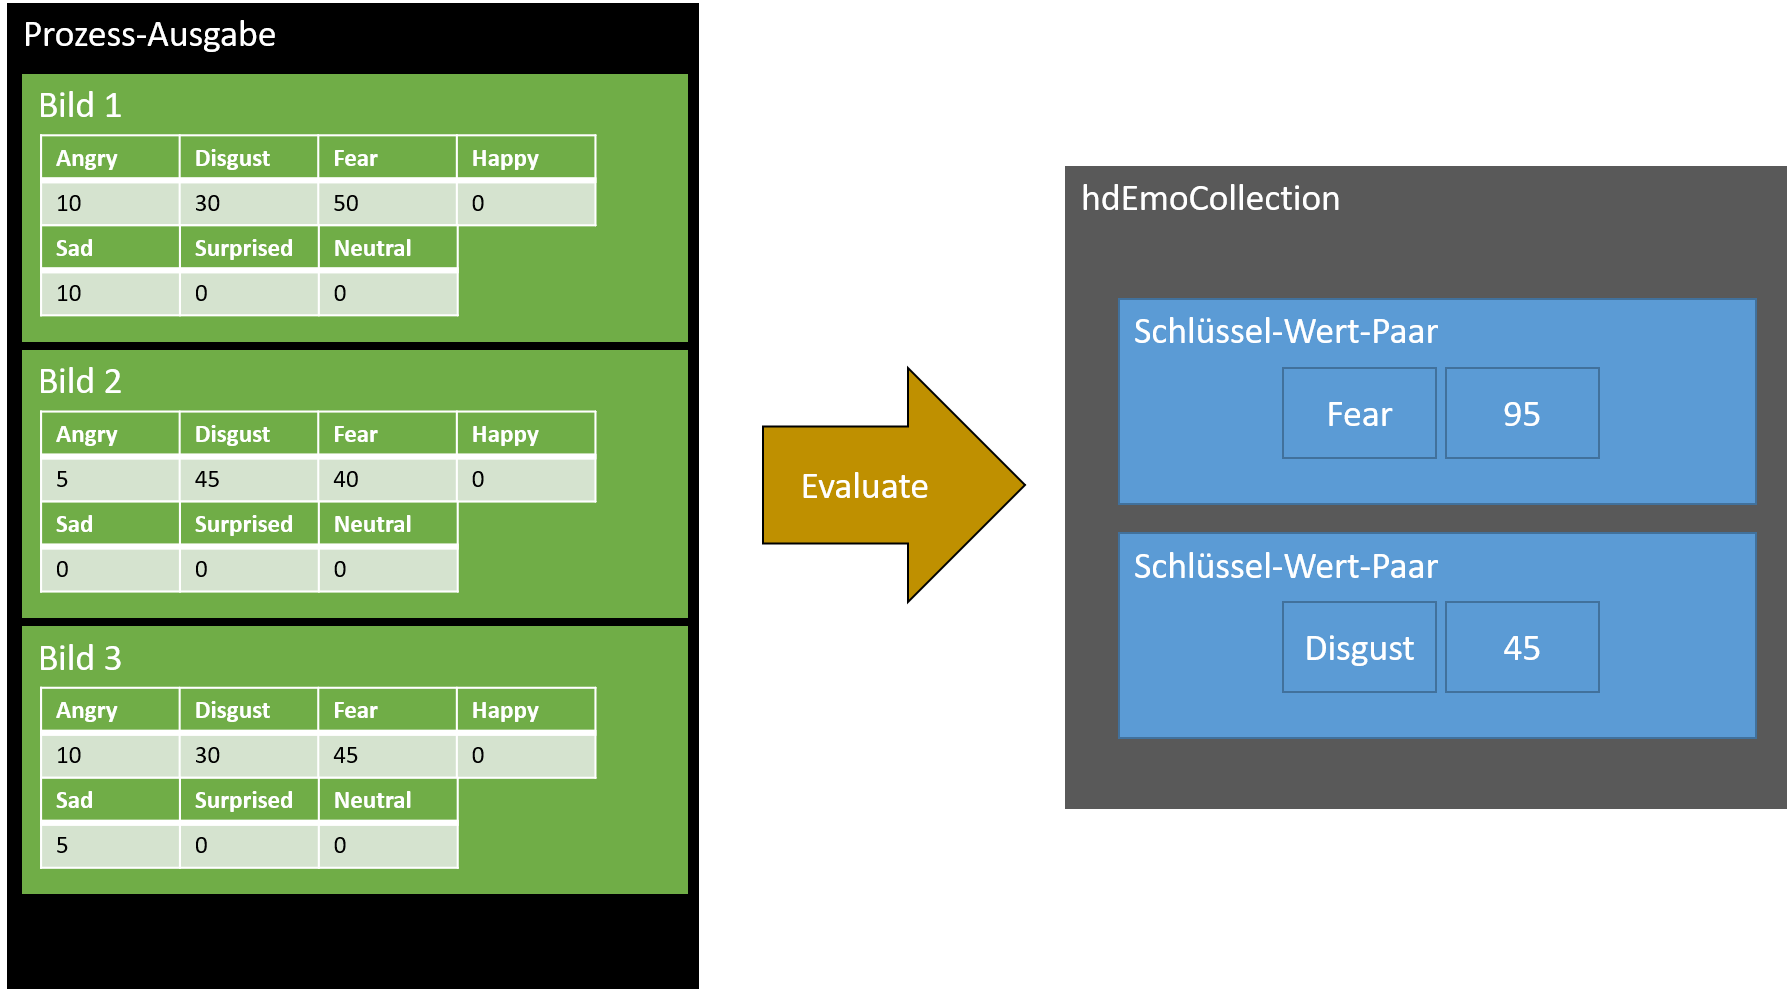
\includegraphics[scale=0.27]{Images/Evaluate_Veranschaulichung.pdf}
 \caption{Visualisierung des Auswertungsvorgangs}
 \label{fig:VisualisierungEvaluation}
 \end{figure}
\subsubsection{GetEmotion}
Diese Funktion liefert das Schl\"{u}ssel-Wert-Paar der \textit{hdEmoCollection}, welches den h\"{o}chsten Wert und somit auch die h\"{o}chste Gewichtung enth\"{a}lt. Tritt der Fall ein, dass die Emotion \textit{„Neutral“} und eine beliebig andere Emotion, beispielsweise \textit{„Happy“}, den gleichen und h\"{o}chsten Wert aufweisen, liefert die \textit{GetEmotion}-Funktion \textit{„Happy“}. Bei \textit{„–Neutral“} handelt es sich um keine vom Benutzer zu fordernde Emotion und somit rechtfertigt sich diese Sonderregelung.

%Lukas
\subsection{Regul\"{a}re Ausdr\"{u}cke in der Ergebniserkennung}
In der Klasse \textit{EmotionTableInterpreter} werden drei Regul\"{a}re Ausdr\"{u}cke benutzt, um die Ergebnisse des Python-Skripts, die als Konsolenausgabe vorliegen, in das Programm zu importieren. Zwei dieser Ausdr\"{u}cke werden zur Erkennung verwendet, der dritte l\"{o}scht Steuerzeichen, die im Eingabestring m\"{o}glicherweise vorhanden sind. Die \texttt{System.Text.RegularExpressions}-Bibliothek bindet die Funktionalit\"{a}t zur Verwendung der Regul\"{a}ren Ausdr\"{u}cke ein.
\subsubsection{Begriffsdefinitionen}
\begin{itemize}
\item[-] Eingabestring: String, dessen Inhalt auf \textit{Matches} durchsucht wird.
\item[-] Match (\textit{plural: Matches}): Teilstring(s) des \textit{Eingabestrings}, der mit dem \textit{Pattern} \"{u}bereinstimmt.
\item[-] Pattern: Regul\"{a}rer Ausdruck
\item[-] Subpattern: Teil eines Regul\"{a}ren Ausdrucks, der benannt wird, um leichter auf ihn zugreifen zu k\"{o}nnen. Einzelne Subpattern k\"{o}nnen auch gematcht werden. 
\end{itemize}
\subsubsection{Regul\"{a}re Ausdr\"{u}cke f\"{u}r die Prozessausgabe}
Die einzelnen Pattern zur Auswertung der Ausgabe werden im Folgenden erkl\"{a}rt.
\subsubsection{patternFaceFoundCount}
Das Pattern \texttt{(Faces found:  (?<FacesFoundCount>[0-9]*))\{1\}} hat den Zweck, die Anzahl der erkannten Gesichter in einem Bild auszulesen. Das Subpattern \texttt{((?<FacesFoundCount>[0-9]*))\{1\}} mit dem Namen \textit{FacesFoundCount} hat als Match eine Zahl aus dem Intervall $\left[0;9\right] \in \mathbb{N}$ und gibt diese bei einem Aufruf zur\"{u}ck. Dieser Wert wird verwendet, um zu entscheiden, ob die vom Modell erzeugten Daten im \textit{EmotionTableInterpreter} ausgewertet werden sollen, oder nicht. Im Abschnitt \"PrepareModel - Konstruktor\" findet sich eine genauere Erkl\"{a}rung.
\subsubsection{patternArray}
Der erste Teil des Patterns hei{\ss}t\textit{SinglePicOutput}. Dieses Subpattern umfasst das gesamte Pattern und soll den 
Zugriff auf den Gesamtoutput eines einzelnen Bildes vereinfachen. Direkt nach der Benennung des Subpatterns beginnt 
das erste Array, dessen Zahl auf dem Index 0 die erkannte Emotion anzeigt. Auf diese Zahl kann sp\"{a}ter mit dem Subpattern 
\texttt{(ar+ay([(?<HighestEmotionIndex>[0-6])} zugegriffen werden.  Ebenso liefert es so den Index im zweiten Array, 
welches die Gewichtung der vom Netz erkannten Emotion enth\"{a}lt. Die restlichen sechs Elemente des Arrays werden nicht in 
einem Subpattern erfasst. Das Pattern muss sie trotzdem erkennen, da  sonst die Erkennung des zweiten Arrays 
schwieriger ist. Dies erfolgt mit dem folgenden Abschnitt: \texttt{([,][ ]*[0-6])*][, dtype=int[32|64]*]*)[,][]*}. Der Abschnitt 
erkennt eine unbekannte Anzahl an Zahlen aus dem Intervall $\left[0;6\right] \in \mathbb{N}$, denen jeweils ein Komma 
folgt. Zwischen dem Komma der letzten Zahl und der n\"{a}chsten Zahl kann sich wiederum eine unbekannte Anzahl an 
Leerzeichen befinden.
Die Gewichtungen im zweiten Array, genannt \texttt{(?<EmotionWeightArray>} werden als Flie{\ss}kommazahlen 
dargestellt. Niedrige Wahrscheinlichkeiten werden mit Hilfe der Exponentialschreibweise ausgegeben. Dies kann zu Zahlen 
wie \texttt{2.8267652e-05} (=> \texttt{2.8267652 $\cdot$ 10$^{-5}$}) f\"{u}hren. Da diese Zahlen potentiell alle das Gewicht 
f\"{u}r die h\"{o}chste erkannte Emotion darstellen k\"{o}nnen, werden sie alle getrennt mit Hilfe von eigenen Subpattern erkannt, 
damit einfach auf sie zugegriffen werden kann. Dies wird im Abschnitt \"Ablauf\" eingehender besprochen. Die Subpattern 
f\"{u}r die Flie{\ss}kommazahlen sind gleich aufgebaut. \texttt{(?<EmotionWeightArray2>[0-9]*[.]*[0-9]*[e]*[-|+]*[0-9]*)} 
erkennt die Gewichtung an der dritten Stelle im Array. Die Zahl ist in sechs Bereiche unterteilt, die jeweils den Anteil vor und  
nach dem Komma und dem \textit{e} der Exponentialschreibweise, sowie das Komma und das  \textit{e} selbst darstellen. 
Jeder Teil des Subpatterns ist so gestaltet, dass die einzelnen Teile nicht im Eingabestring enthalten sein m\"{u}ssen.

\subsubsection{Ablauf}
In diesem Teil soll erkl\"{a}rt werden, wie die Regul\"{a}ren Ausdr\"{u}cke zur Datenextraktion genutzt werden. Zuerst werden aus dem Eingabestring alle Steuerzeichen entfernt. Da die Erkennung dieser aufgrund
 von Performance-, Stabilit\"{a}\"{a}ts- und \"{u}bersichtlichkeitsgr\"{u}nden nicht im Pattern \textit{patternArray} enthalten sind. Daraufhin wird auf der Grundlage von \textit{patternFaceFoundCount}
 der Eingabestring durchsucht und entsprechende Daten als Variable des Typs \textit{MatchCollection} gespeichert. Die Daten, die gegen \textit{patternFaceFoundCount} gematcht wurden, werden mit dem Namen
 des Subpatterns wie folgt aufgerufen: \texttt{MatchCollection[Index].Groups[NameDesSubpattern].Value}. Diese Daten sind vom Typ \textit{string} und k\"{o}nnen  in eine anderen Typ konvertiert werden. Hier ist dies notwendig, um auf die Anzahl der erkannten Gesichter zuzugreifen und zu entscheiden, wie weiter vorgegangen werden soll.
 Danach wird der Eingabestring mit Hilfe des Patterns \texttt{patternArray} noch einmal gematcht und die einzelnen \textit{SinglePicOutput}-Subpatterns als \textit{strings} an die \textit{Evaluate}-Methode \"{u}\"{u}bergeben. Dort wird zuerst das Subpattern \texttt{HighestEmotionIndex} ausgelesen und auf die Subpatterns des \texttt{EmotionWeightArray} angewendet, um den durch das Modell zugewiesenen Wert der Gewichtung der h\"{o}\"{o}chsten Emotion des Bildes auszulesen. Jetzt wird auf den Namen der als wahrscheinlichsten erkannten Emotion aus dem Member \textit{string [] emoDefinition} mit dem erkannten Wert des Subpatterns \texttt{HighestEmotionIndex} zugegriffen. Die danach stattfindenden Berechnungen werden in den Abschnitten \textit{Evaluate} und \textit{GetEmotion} dargestellt. 


\section{Benutzeroberfläche}

\subsection{Werkzeuge Oberflächenlogik} %????
\subsubsection{C\#}
Was ist C\#? \\
C\# ist eine typsichere, objekt-orientierte Programmiersprache. Sie wurde 2001 von Anders Hejlsberg im Auftrag von Microsoft entwickelt. Es ist eine plattformunabhängige Sprache, wurde aber für die .NET-Umgebung entworfen. C\# basiert auf den Programmiersprachen C und C++ und ist eng verwandt mit Java\cite{Shildt2010}.\\
Warum haben wir C\# gewählt? \\
Da C\# grundlegend mit denen von uns bereits im Zuge des Studiums gelernten Programmiersprachen C sowie C++ verwandt ist, aber zusätzlich eine zeit- und aufwandsarme Umsetzung des MVVM Schema bietet, haben wir uns für diese Sprache entschieden.

\subsubsection{.NET Framework} 
Das .NET Framework wurde 2002 von Microsoft entwickelt. Ziele des Frameworks wie auch der Plattform .NET sind unter anderem Kompatibilität zwischen verschiedenen Plattformen, Zusammenführung bisher inkompatibler Microsoft Technologien und Verbesserung veralteter Standards. \cite{DotNet}
\\
Einer der zwei Hauptbestandteile des .NET Framework ist die .NET Klassenbibliothek. Damit ist es möglich sowohl schnell einfache Anwendungen als auch Unternehmensanwendungen im großen Stil zu entwickeln. Auch Umsetzungen der „Gang of Four“-Pattern, sowie andere Strukturen, wie das von uns benutzte Model-View-Viewmodel-Strukturmuster sind im .NET Framework enthalten.  \\

Die Objektorientierung von C\# ist auch in der .NET Klassenbibliothek fortgeführt, so das jedes Element als Objekt, von der Instanzen bestehen können, behandelt wird. Diese Objekte können von wiederum anderen Objekten erben, d.h. diese um Parameter und Funktionen erweitern. Die Wurzel der .NET-Klassenhierarchie ist die Klasse Objekt von der alle anderen Klassen ableiten. Auf diese Weise entsteht eine mehr oder weniger ausgeprägte Baumstruktur\cite{Kühnel}. \\

Die zweite Komponente ist die Common Language Runtime (CLR). Die CLR ist die Umgebung, in der die .NET-Anwendungen ausgeführt werden. Diese Umgebung beinhaltet unter anderem Dienste wie:
\begin{itemize}
\item Der Class Loader, um Klassen in die Laufzeitumgebung zu laden
\item Der Type Checker, der unzulässige Typkonvertierungen unterbindet
\item Der Garbage Collector, der eine  automatische Speicherbereinigung anstößt, wenn Objekte nicht mehr benötigt werden
\item Der Exception Manager, der die Ausnahmebehandlung unterstützt
\item Die Debug Machine zum Debuggen der Anwendung, und viele mehr \cite{Kühnel}
\end{itemize}
\subsubsection{WPF}
Was ist WPF? \\
Mit dem .NET Framework 3.0 wurde 2006 eine neue Programmierschnittstelle für Windows-Anwendungen eingeführt, die sich Windows Presentation Foundation (WPF) nannte. \\
Mit WPF lassen sich grafische Benutzeroberflächen entwickeln. Im Gegensatz zum Vorgänger, der WinFormAPI, trennt WPF die Präsentations- und Geschäftslogik. Dadurch wird eine Umsetzung des Model-View-Viewmodel-Strukturmuster möglich.  \\
Die Benutzeroberfläche (View) wird mit einer an XML angelehnten Sprache beschrieben. Diese Sprache heißt eXtensible Application Markup Language (XAML). Dadurch ist es möglich, die Beschreibung der Benutzeroberfläche strikt vom logischen Code zu trennen\cite{Kühnel}. \\
Warum haben wir WPF gewählt?
Durch die Trennung von Präsentations- und Geschäftslogik ist eine übersichtliche Strukturierung des Projekts möglich. Da unser Team auf verschiedene Kernthemen unterteilt ist, die im Großen und Ganzen der Aufteilung des WPF entspricht, lag die Wahl auf WPF sehr nahe.

\subsubsection{MVVM}
Was ist MVVM? \\
Das Model-View-Viewmodel-Strukturmuster (MVVM) ist eine Variante des Model-View-Controller-Muster (MVC). Hier entspricht das Viewmodel dem Controller und übernimmt dessen Funktion. \\
\begin{itemize}
\item Das Model (Datenmodell) stellt alle für die Verarbeitung einer Anforderung notwendigen Daten und Informationen bereit.
\item Der Controller (Viewmodel) steuert die Verarbeitung, er nimmt die Anforderungen entgegen, befüllt das Model und gibt danach die Kontrolle an die View weiter.
\item Die View (Ansicht) ist für die Darstellung der Informationen, die sie in Form des Models vom Controller erhält, zuständig\cite{Kühnel}.
\end{itemize}

\subsection{Aufbau und Ablauf der Oberflächenlogik}
Der Einstiegspunkt der Oberfläche und sogleich das einzige Fenster des Programms ist das sogenannte "{}MainWindow"{}. In WPF kann man Fenster in unterschiedliche Dateien aufteilen. Im Falle des "{}MainWindows"{} wurde hierbei eine Unterteilung in eine ”{}XAML"{} und eine “{}C Sharp"{} Datei durchgeführt. Die "{}XAML"{} Datei legt das Layout des Fensters sowie alle Bezeichner der Komponenten fest, während die "{}C Sharp"{} Datei für die Interaktivität der Komponenten des Fensters sorgt. 
\paragraph{}
Beim Starten der GUI müssen zuerst alle Komponenten des "{}MainWindows"{} initialisiert werden. Vorher kann kein Code mit diesen Komponenten arbeiten, da diese ansonsten noch nicht existieren. Anschließend wird in einem neuen "{}Thread"{} die Logik des Programms gestartet.
\paragraph{}
In WPF läuft die GUI innerhalb des "{}Hauptthreads"{}. Dieser behandelt Interaktionen mit dem User, wie beispielsweise Eingaben oder das Schließen des Fensters. Falls man nun Code innerhalb des "{}Hauptthreads"{} ausführen würde, könnte das System auf keinerlei Eingaben des Users mehr reagieren, da der Thread, der dafür zuständig sein sollte, durch den programmierten Code blockiert wird. Aus diesem Grund muss man für die spezielle Programmlogik einen seperaten Thread erstellen. Dabei ist zu beachten, dass dieser Thread als "{}Background-Thread"{} konfiguriert wird. Das bedeutet, dass bei Schließen des Programms und damit auch Terminieren des "{}Hauptthreads"{}, der seperate Thread ebenfalls terminiert wird. Würde man diese Konfiguration unterlassen, bleibt das Programm nach Schließen der Oberfläche weiterhin aktiv.
\paragraph{}
Innerhalb des neuen Threads wird eine Instanz von "{}MainWindowViewModel"{} erstellt. Das "{}MainWindowViewModel"{} stellt die Schnittstelle zwischen der tatsächlichen GUI (View) und der da hinterliegenden Logik und Daten (Model). Das "{}ViewModel"{} ruft die benötigten Abhängigkeiten der Oberfläche auf (beispielsweise das neuronale Netz), verarbeitet deren Antwort und aktualisiert die Oberfläche um den User über den derzeitigen Zustand des Programms zu informieren. 
\paragraph{}
Der Einstieg des "{}ViewModels"{} ist die Erkennung des Users. Hierbei kann es zu unterschiedlichen Fällen kommen. Werden mehrere User erkannt oder wird kein User erkannt, bricht das Programm die Analyse ab und probiert es zu einem späteren Zeitpunkt erneut. Falls jedoch ein einziges Gesicht erkannt wurde, startet das Programm eine Spielrunde.

\paragraph{}
Bei der Änderung der GUI durch das "{}ViewModel"{} muss ebenfalls ein wichtiger Punkt beachtet werden. Falls man eine Änderung auf der GUI durchführen möchte, beispielsweise die Änderung des Textes eines Labels, kann dies nicht im "{}Background-Thread"{} durchgeführt werden. Dies ist nur innerhalb des Hauptthreads erlaubt. WPF bietet Möglichkeiten um Aktionen für den Hauptthread einzustellen, die anschließend dort ausgeführt werden. Dies wird vielfach innerhalb das "{}MainWindowViewModels"{} aufgerufen.
\paragraph{}
Eine Spielrunde startet durch das randomisierte Generieren eines Emojis. Hierbei wird zwischen "{}Wütend"{}, "{}Ekel"{}, "{}Angst"{}, "{}Freude"{}, "{}Neutral"{}, "{}Traurig"{} und "{}Überrascht"{} ausgewählt. Diese Emojis sind als externe Bilder gespeichert und werden bei Bedarf geladen und in der GUI angezeigt. Anschließend wird der User gebeten die Emotion des Emojis nachzumachen. Nach einer gewissen Zeit, wird ein Bild des Users aufgenommen und an einem vorgegebenen Ort als eine JPEG Datei gespeichert. Das neuronale Netz übernimmt nachfolgend den Programmablauf und analysiert das gespeicherte Bild.
\paragraph{}
Diese Analyse kann zu drei unterschiedlichen Fällen führen. Die erste Möglichkeit ist, dass kein Gesicht erkennbar war, da der User beispielsweise das Spiel verlassen hat. Hierbei wird eine Information ausgegeben und das System versucht erneut in regelmäßigen Abständen ein Gesicht für eine neue Spielrunde zu erkennen. Die zweite Möglichkeit ist, dass das neuronale Netz mehrere Gesichter erkannt hat. In diesem Fall wird eine Fehlermeldung ausgegeben und eine neue Spielrunde gestartet. Die letzte Möglichkeit ist, dass nur ein User erkannt wird. Das neuronale Netz gibt im Erfolgsfall eine Prozentzahl an, die spezifiziert wie gut eine bestimmte Emotion erkannt wurde. Wichtig ist das nur die Emotion mit der größten Prozentzahl verarbeitet wird. Falls diese mit der randomisierten Emotion übereinstimmt, bekommt der User die Prozentzahl auf sein Punktekonto gutgeschrieben. Andernfalls bekommt der User keine zusätzlichen Punkte und die nächste Runde beginnt.



\subsection{WebCam}
Die Webcam wird von der MainWindow Klasse gesteuert. Sie ist über die Using-Direktive WebEye.Controls.Wpf eingebunden.   Sobald das Fenster nach dem Start der Applikation geladen hat, wird die Webcam über die Funktion
 OnWindowLoaded(object sender, RoutedEventArgs e) initialisiert. In der Funktion wird dabei zuerst eine Liste aller Webcams, die dem System verfügbar sind, erstellt.  Die Webcam an der erster Stelle dieser Liste wird anschließend mit webCameraControl.StartCapture(cameras[0]) 	gestartet. Dieser Kamerastream wird in der MainWindowViewModel Klasse dazu benutzt Bilder für das Neuronale Netz zu machen. Dies geschieht im fünf Sekunden Takt wenn kein Gesicht erkannt wurde und im elf Sekunden Takt wenn das Spiel gestartet wurde. Mithilfe von img = BitmapConverter.ConvertToBitmapSource(MainWindow.main.webCameraControl.GetCurrentImage()) wird das aktuelle Webcam Bild 
als Objekt des Typs BitmapSource gespeichert, was anschließend beim Verwenden des neuronalen Netzes genutzt wird.


\chapter{Fazit, Diskussion und Zusammenfassung}
\section{Ergebnisse}
\subsection{Ergebnisse in der Programmierung}
Die Klassen \textit{PrepareModel}, \textit{EmotionTableInterpreter} und \textit{ReturnObject} wurden erstellt und so miteinander verbunden, dass sie einen externen Prozess starten k\"{o}nnen und die Ausgabe dieses Prozesses in den eigenen Prozess einlesen, verarbeiten und weitergeben. Die Klasse \textit{PrepareModel} stellt je ein Objekt der Klassen \textit{System.Diagnostics.Process},  \textit{ReturnObject} und \"{u}bergibt sie einem ebenfalls bereitgestellten Objekt der Klasse  \textit{EmotionTableInterpreter}.
In der Klasse \textit{EmotionTableInterpreter} wird das \textit{System.Diagnostics.Process}-Objekt gestartet. Diese Aktion startet eine Instanz des externen Programms \textit{Python.exe}. In diesem Programm werden vom aufrufenden Programm zur Verf\"{u}gung gestellte Bilder mit Hilfe eines von Lewe Ohlsen \cite{LeweOhlsen} erstellten und trainierten neuronalen Netzes auf der Grundlage des FER+-Trainingsdatensatzes aus. Diese Daten werden als Objekt des Typs \textit{string} wieder in die Klasse \textit{EmotionTableInterpreter} eingelesen und dort von selbst entwickelten regul\"{a}ren Ausdr\"{u}cken mit Hilfe der Systembibliothek \textit{System.Text.RegularExpressions} auf die relevanten Daten untersucht und an das \textit{ReturnObject}-Objekt \"{u}bergeben. Dieses kann dann weiter verarbeitet werden. Teile des in \textit{Python} geschriebenen, zum neuronalen Netz geh\"{o}rigen Skripts wurden auf die Bed\"{u}rfnisse des Programms angepasst. So ruft nun das \textit{Python}-Skript abgespeicherte Bilder auf, anstatt dauernd den Input einer Webcam zu verarbeiten. Zus\"{a}tzlich wurde der Aufruf der GUI des Skripts gel\"{o}scht.
\subsection{Ergebnisse in der Verwendung aller Programmteile}
Vor der ersten Ausf\"{u}hrung des Programms m\"{u}ssen mehrere Punkte beachtet werden.
\begin{itemize}
\item[-] Es muss Python 3.6 oder h\"{o}her auf dem Zielger\"{a}t installiert sein.
\item[-] Python muss in die PATH-Variable des Zielger\"{a}tes eingef\"{u}gt worden sein.
\item[-] Das Netz muss wie in der Anleitung\cite{LeweOhlsenGit} von Lewe Ohlsen mit dem Kommandozeilenbefehl \textit{python pip -install -r ''requirements.txt''} installiert werden.
\end{itemize} 
Im Betrieb des Programms fallen verschiedene Besonderheiten mit Bezug zum neuronalen Netz auf, die vor einer Installation bedacht werden sollten.
\begin{itemize}
\item[-] Die ''Positiven'' und die ''neutrale'' Emotion werden am Einfachsten erkannt. ''Negative'' Emotionen werden seltener erkannt.
\item[-] Manchmal werden Gesichter in Strukturen erkannt, die kein Gesicht sind. Verschiedene Experimente konnten keine Struktur hinter diesem Verhalten aufzeigen.
\item[-] Personen, die Brillen tragen m\"{u}ssen diese vor dem Spielstart abnehmen, da die Brillen das Ergebnis der Auswertung ver\"{a}ndern und meistens die ''Emotion'' \textit{''\"{U}berrascht''} erkannt wird. 
\end{itemize}
\section{Diskussion der Ergebnisse}
Im programmierbaren Teil finden sich keine \"{U}berraschungen. Alle Teile der Sprache \textit{C\#} haben wie erwartet miteinander funktioniert und die gew\"{u}nschten Ergebnisse geliefert. Der einfache Aufruf von \textit{Python}-Skripten aus dem Programm heraus war eine erfreuliche \"{U}berraschung, die sehr viel Entwicklungsarbeit ersparte. Die regul\"{a}ren Ausdr\"{u}cke kommen im Allgemeinen nicht sonderlich gut mit im Eingabestring vorhandenen Steuerzeichen zurecht. Dieser Fehler wurde erst in der Testphase erkannt und behoben werden. Der aktuell gew\"{a}hlte Weg ist zwar nicht optimal, entfernt aber Steuerzeichen zuverl\"{a}ssig. Leider war die Ausgabe des mit \textit{CK+} trainierten Models nicht so einfach auswertbar wie die Ausgabe des mit \textit{FER+} trainierten Models. Da \textit{CK+} manchmal als bessererer Trainingsdatensatz zur Emotionserkennung eingestuft wird, beeinflu{\ss}t dieses Ereignis die Daten der Auswertung in ihrer Qualit\"{a}t negativ. Vor allem die Erkennung der ''negativen'' Emotionen ist im \textit{CK+}-Datensatz erheblich verbessert.  Nicht \"{u}berraschend waren die Effekte, die erzeugt werden k\"{o}nnen, wenn ein Bild eines Brillentr\"{a}gers ausgewertet wird. Aufgrund der Arbeitsweise des neuronalen Netzes werden Brillen als ''aufgerissene Augen'' erkannt. Das kann ein Nachteil f\"{u}r Brillentr\"{a}ger sein, die den angezeigten Emoji vielleicht nicht erkennen k\"{o}nnen. Solche Nachteile m\"{u}ssen mit einer geschickten Platzierung der Kamera ausgeglichen werden.
\section{Zusammenfassung}
Unser gemeinsames Ziel als NN-Gruppe war es, dem neuronalen Netz von Lewe Ohlsen ein Ger\"{u}st zu geben, mit dem es ohne Probleme von einem \textit{C\#}-Programm aufgerufen und sein Output eingelesen werden kann.%32
Wir verwendeten die M\"{o}lichkeiten, die uns von der Sprachen \textit{C\#} und Python zur Verf\"{u}gung gestellt wurden. Besonders hervorzuheben sind \textit{System.Text.RegularExpressions} und \textit{System.Diagnostics}, welchen den Start, das Auslesen und das Auswerten des Ergebnisses eines von diesem Programm gestarteten Prozesses erm\"{o}lichen. OpenCV und Tensorflow werden genutzt, um die auszuwertenden Bilder vorzubereiten und zu verarbeiten.%51
Es wurden drei Klassen geschrieben, die einen bestimmten externen Prozess starten und auswerten k\"{o}nnen. Das Programm des Prozesses ist in einer anderen Programmiersprache geschrieben und die Ergebnisse m\"{u}ssen von den Klassen als String eingelesen und mit den geeigneten Mitteln ausgewertet werden. Die Ergebnisse des Python-Prozesses h\"{a}ngen in besonderem Ma{\ss}e vom gew\"{a}hlten Model ab. Je nach dem mit welchem Datensatz das Model trainiert wurde, werden Gesichtsausdr\"{u}cke unterschiedlich bewertet und ausgegeben. %68
Die ausgewerteten Daten werden mit regul\"{a}ren Ausdr\"{u}cken verglichen und von geeigneten Funktionen auf die H\"{a}ufigkeit der aufgetretenen Emotion untersucht. Diese Information wird danach in einem Objekt an die aufrufenden Klassen zur\"{u}ckgegeben.%31
\newline
Aufgrund der Daten und der Umsetzung l\"{a}sst sich schlussfolgern, dass das Programm erfolgreich Gesichtsausdr\"{u}cken ''Emotionen'' erfolgreich zuordnen kann und die Ergebnisse dieser Zuordnung an aufrufende Klassen und Programme ausgeben kann.
 




% Literaturverzeichnis
\printbibliography


% Anhang
\appendix

 
\end{document}
